\problemname{Balanced Cut}

Professor Anna van Lier is preparing to give a lecture on balanced binary search trees.
Recall that these are binary trees with two properties:
\begin{itemize}
\item \emph{Balanced tree:} For every node, the height of its left subtree and the height
of its right subtree differ by at most $1$.  For instance in
Figure~\ref{fig:avltree}, the left and right subtrees of node $7$ have
heights $2$ and $1$, respectively.  If a node does not have a left (or
right) subtree then that subtree is considered to have height $0$.
\item \emph{Search tree:} Each node has a value. The value of a node is greater than all the values
in the left subtree of the node, and smaller than all the values
in the right subtree of the node.  For instance in
Figure~\ref{fig:avltree}, the left subtree of node $7$ contains the
values $4$, $5$ and $6$ which are all smaller than $7$.
\end{itemize}

Anna got a picture of such a tree from a colleague.  This tree has $n$ nodes with the values $1$ to $n$.
However, it turns out to be too big to fit on her slides so she would like to make it smaller.
In particular, she would like to erase some nodes from the tree such
that it has exactly $k$ remaining nodes.
Whenever she erases a node, she also erases the subtrees of that node.
Of course, the resulting tree must still be a balanced binary search tree.

For pedagogical purposes, Anna would like the node values in her final
tree to be small.  Therefore, she wants the list of the $k$ remaining
node values to be the lexicographically smallest possible.  For
example she would prefer a tree containing values $2, 5, 9$ over a tree
containing values $2, 6, 7$.

As Anna is far too busy doing more important things, the task of
finding which nodes to erase falls upon one of her teaching assistants, i.e., you.

\begin{figure}[!h]
\begin{center}
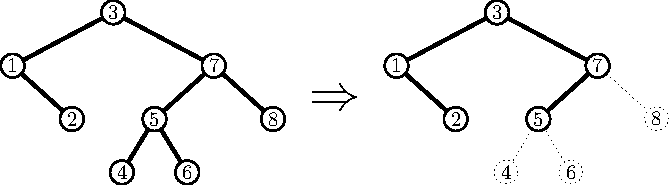
\includegraphics[width=0.9\textwidth]{sample1}
\caption{Illustration of Sample Input 2 and its solution.}
\label{fig:avltree}
\end{center}
\vspace{-1cm}
\end{figure}


\section*{Input}

The input consists of:
\begin{itemize}
  \item One line with two integers $n$ and $k$ ($2 \leq n \leq 5 \cdot 10^{5}$, $1 \leq k \leq n - 1$), the
    number of nodes in the tree and the number of nodes to keep.
\item $n$ lines, the $i$th of which contains an integer $p_i$ ($1\leq p_i \leq n$ or
	$p_i = -1$), the parent of the node with value $i$ or $-1$ if the node with value $i$ is the root.
    % Each value from $1$ to $n$ (inclusive) occurs at most twice and $-1$ occurs exactly once.
\end{itemize}

It is guaranteed that the given tree is a balanced binary search tree.

\section*{Output}

Output a single line with a binary string of length $n$.
The $i$th character should be `\texttt{1}' if the node with value $i$ should be kept,
and `\texttt{0}' if it should be erased.
